\documentclass{article}
\usepackage{graphicx}
\usepackage[utf8]{inputenc}
\usepackage{amssymb}
\usepackage{caption}
\usepackage{subcaption}
\usepackage{array}
\usepackage{tabularx}

\title{\textbf{\Huge Image Compression Using Discrete Wavelet Transform}}
\author{\Large Anitha Pappu: 202SP002, Kranti Kumari: 202SP011 \\ Under the guidance of Dr. Aparna P\\\\ Department of Electronics and Communication Engineering\\ National Institute of Technology, Surathkal\\  Karnataka-575025, India}
\date{January 2021}

\begin{document}

\maketitle

\begin{flushleft}
\textbf{\large 1. Abstract}
\end{flushleft}

The swift development in digital technology has increased the use of images in practically all the applications. The extensive use of these images have raised the need of image compression, so as to save memory and transmission bandwidth 
of the medium. This project focuses on the grayscale image compression using Discrete Wavelet Transform (DWT). The Wavelet Algorithm contains transformation process, quantization process, and lossy entropy coding. The main purpose of this project is to maintain the quality of image after the image compression process using Wavelet Algorithm. Besides that, it can produce high compression performance and minimize the amount of the image data so that it can be stored effectively.\\

\begin{flushleft}
\textbf{\large 2. Introduction}
\end{flushleft}

Image compression is a process of reducing the amount of data required to represent a particular amount of information by exploiting the redundancy within the data. The reduction in the data reduces the number of bits required to store or transmit the image over digital media.\\\\
Image compression is also of two types: First, Lossless, in which the reconstructed image is exact replica of the original image. Methods for lossless image compression includes: Entropy coding, Huffman coding, Bit-plane coding, Run-length coding and LZW (Lempel Ziv Welch) coding. Second, Lossy, where the reconstructed image is not an exact replica of the original image. Methods for lossy compression include: Fractal compression, Transform coding, Fourier-related transform, DCT (Discrete Cosine Transform) and Wavelet transform.\\
In lossy compression, there is always some loss in the data. The extent of compression is more in lossy compression techniques compared to lossless compression techniques, but the superiority of reconstructed image is good in lossless compression.\\\\

\begin{flushleft}
\textbf{\large 3. Image Compression and Reconstruction}
\end{flushleft}

In general, there are three essential stages in a Wavelet transform image compression system: transformation, quantization and entropy coding. Figure 1 depicts the encoding and decoding processes in which the reversed stages are performed to compose a decoder. The dequantization is the only different part in the decoding process and it followed by an inverse transform in order to approximate the original image. 

\begin{figure}[htp]
    \centering
    \Large\includegraphics[width=12cm]{BlockDiagram.PNG}
    \caption{Block Diagram of Encode and Decode Process by using Wavelet Transformation Algorithm}
    \label{fig:BlockDiagram}
\end{figure}


\begin{flushleft}
\textbf{\large 3.1. Performance Indicator }
\end{flushleft}

\begin{flushleft}
\textbf{3.1.1. Compression ratio}
\end{flushleft}

The compression that is achieved can be quantified by the compression ratio given by the following formula:
\[Compression Ratio = \frac{Uncompressed Size}{Compressed Size}\]

Compression ratio is the ratio of numbers of bits required to represent original image to the number of bits required to represent compressed image.

\begin{flushleft}
\textbf{3.1.2. Mean Square Error (MSE)}
\end{flushleft}

Mean square error is the cumulative squared error between the compressed image and the original image.

\[MSE = \frac{1}{MN}\sum_{y=1}^M \sum_{x=1}^N [I(x,y) - I'(x, y)]^2\]

\begin{flushleft}
\textbf{3.1.3. Peak Signal to Noise Ratio (PSNR)}
\end{flushleft}

Peak Signal to Noise Ratio is the ratio if maximum power of the signal and the power of unnecessary distorting noise.

\[PSNR = 20 * \log_{10}{[\frac{255}{\sqrt{MSE}}}]\]\\

\begin{flushleft}
\textbf{\large 4. Wavelet Transform}
\end{flushleft}

Wavelets are functions defined over a finite interval and having an average value of zero.\\
The discrete wavelet transform is analogous to the discrete Fourier transform. Now, instead of using trigonometric functions, different families of basis functions are used. A function called the wavelet or mother wavelet, usually denoted by $\psi$, and another function called the scaling or father scaling function, typically represented by $\phi$, are the basis of a wavelet family. A countably infinite set of wavelet functions (commonly known as daughter wavelets) can be generated using dilations and shifts of the first two functions:
\begin{figure}[htp]
    \centering
    \Large\includegraphics[width=4cm]{Function.PNG}
    \label{fig:Function}
\end{figure}\\
where m, k $\in$ $\mathbb{Z}$\\

\begin{flushleft}
\textbf{\large 5. Proposed Compression Method using DWT}
\end{flushleft}

Lossless compression produces a compression ratio of nearly 0.5. In our project, we are using Wavelet Scalar Quantization (WSQ), which is a lossy wavelet compression. It is a lossy compression, though the loss of information is not perceived by human eye.
The Wavelet Scalar Quantization (WSQ) algorithm is among the first successful wavelet-based image compression algorithms. This algorithm is capable of achieving compression ratios in excess of 10-to-1 while retaining excellent image quality. 
Quantization is the process of mapping each wavelet coefficient to an integer value, and is the main source of compression in the algorithm. By mapping the wavelet coefficients to a relatively small set of integer values, the complexity of the data is reduced, which allows for efficient encoding of the information in a bit string. Further, a large portion of the wavelet coefficients will be mapped to 0 and discarded completely.\\

The steps of the proposed compression algorithm based on DWT are described below:\\
\textbf{I. Decompose}\\
Choose a wavelet; choose a level N. Compute the wavelet. Decompose the signals at level N. \\\\
\textbf{II. Quantize}\\
Maps the wavelet coefficients to a relatively small set of integer values and reduce the complexity of the data.\\\\
\textbf{III. Reconstruct}\\
Compute wavelet reconstruction using the original approximation coefficients of level N and the modified detail coefficients of levels from 1 to N.\\
\begin{flushleft}Figure 2 depicts the LL, LH, HL and HH bands of the input image.\end{flushleft}
\begin{figure}[htp]
    \centering
    \Large\includegraphics[width=10cm]{Decompose.JPG}
    \caption{Subbands for the lena image after one pass through the filter bank}
    \label{fig:Decompose}
\end{figure}

\begin{flushleft}
\textbf{\large 6. Result and Analysis}
\end{flushleft}

The main goal for this system is to maintain the quality of image after the compression process using Wavelet Algorithm.

\begin{flushleft}Compression ratio achieved for different image file formats is shown in table 1: \end{flushleft}
\begin{center}
    \begin{tabular}{ | l | l | l | p{3cm} |}
    \hline
        Image File Format & File Size & Reconstructed Image Size & Compression Ratio\\
    \hline
        JPG  & 97.7 KB  & 62.7KB & 29.262  \\
    \hline
        TIFF  & 205 KB  & 155 KB & 28.978  \\
        
    \hline
    \end{tabular}
\end{center}

\begin{flushleft}Figure 3 depicts the result obtained using our method: \end{flushleft}

\begin{figure}[htp]
  \begin{subfigure}[b]{0.4\textwidth}
    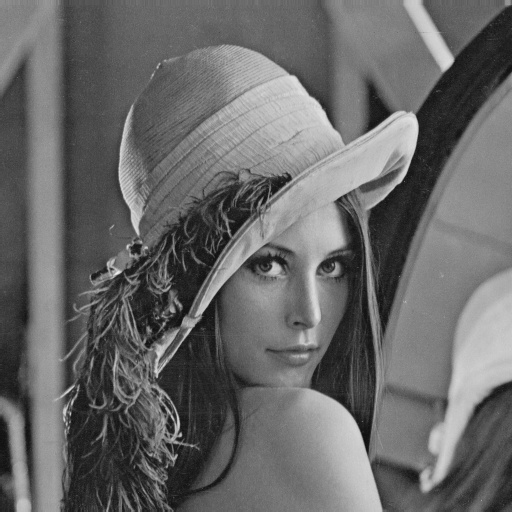
\includegraphics[width=\textwidth]{greyscale_lenna.jpg}
    \caption{Original Lena Image}
    \label{fig:greyscale_lenna}
  \end{subfigure}
  \hfill
  \begin{subfigure}[b]{0.4\textwidth}
    \includegraphics[width=\textwidth]{Compressed_image.jpg}
    \caption{Compressed Lena Image}
    \label{fig:Compressed_image}
  \end{subfigure}
  \caption{Result obtained using our method}
\end{figure}


\begin{flushleft}
\textbf{\large 7. Conclusion}
\end{flushleft}

The wavelet transform can be used as a lossy image compression technique. This technique provides good compression to grayscale images. Wavelet transform is much suitable for low bit rate images. DWT is used as basis for transformation in JPEG 2000 standard. DWT provides high quality compression at low bit rates. The use of larger DWT basis functions or wavelet filters produces blurring near edges in images. This ratio gives an indication of how much compression is achieved for a particular image. The compression ratio typically affected the image quality.\\ 

\begin{flushleft}
\textbf{\large 8. References}
\end{flushleft}

[1] http://www.ijana.in/papers/Paper-2.10.pdf\\

[2] David Salomon Data Compression: The Complete reference, 2nd Edition\\

[3] Anoop Mathew et al, 2009 “Image Compression Using Lifting Based Discrete Wavelet Transform (DWT)” Bharath University, Chennai.\\

[4] S. Sharma and S. Kaur, "Image Compression using Hybrid of DWT, DCT and Huffman Coding," International Journal for Science and Emerging Technologies with Latest Trends, vol. 5, no. 1, pp. 19-23, January 2013.\\

[5] M. Antonini , M. Barlaud and I. Daubechies, "Image Coding using Wavelet Transform”,IEEE Trans. On Image Processing Vol.1, No.2, pp. 205 – 220, APRIL 1992.


\end{document}
